%=================================
%Please do not change this environment
\documentclass{snpyrs}
\usepackage{graphicx}
\textheight 25.cm
\textwidth 17cm
\oddsidemargin -18pt
\evensidemargin 0pt
\topmargin -50pt
\pagestyle{empty}
%================================

\newcommand{\be}{\begin{eqnarray}}
\newcommand{\ee}{\end{eqnarray}}
\newcommand{\ket}{\rangle}
\newcommand{\bra}{\langle}
\newcommand{\del}{\partial}
\newcommand{\pslash}{{p\hspace{-5pt}/}}
\newcommand{\dslash}{{\del \hspace{-5pt}/}}
\newcommand{\zslash}{{z\hspace{-5pt}/}}
\newcommand{\kslash}{{k\hspace{-6pt}/}}
\newcommand{\Thep}{\Theta^+}
\newcommand\gsim{\displaystyle\mathop{>}_{\sim}}
\newcommand\lsim{\displaystyle\mathop{<}_{\sim}}


\begin{document}

%==============================================================
%    Authors and tytle
%
\begin{center}
{\large \bf Evaluation of performance of filtering process of NestDAQ online filter for J-PARC Charm baryon spectroscopy}
\vspace*{0.3cm}

%Authors
First, Last$^{1}$ and Fname, Lname$^{2}$\\
%Address{1}
$^{1}${\it Research Center for Nuclear Physics (RCNP), Osaka University,
Ibaraki, Osaka 567-0047, Japan}\\
%Address{2}
$^{2}${\it Research Center for Nuclear Physics (RCNP), Osaka University,
Ibaraki, Osaka 567-0047, Japan}\\
\end{center}

\vspace*{0.5cm}
%
%==============================================================
%     Main text
%
Brief background and purposes. 
Brief background and purposes.  
Brief background and purposes.  
Brief background and purposes.  
Brief background and purposes.  
Brief background and purposes~\cite{Brambilla:2022ura}.


Methods methods methods. 
Methods methods methods.  
Methods methods methods.  
Methods methods methods.  
Methods methods methods~\cite{Aoki:2021cqa}.



Fig.~\ref{fallapart} shows the process that we study. 
The matrix element is then expressed as 
\be
{\cal M}_{A \to BC} =
-i \sqrt{2} 
\bra BC |  
 \int d^3 x \, g \bar \psi \gamma_5 \psi
e^{-i \vec q \cdot \vec x} 
|A\ket ,
\label{calM1}
\ee

%figure---------------------------------------------
\begin{figure}[h]
\centering
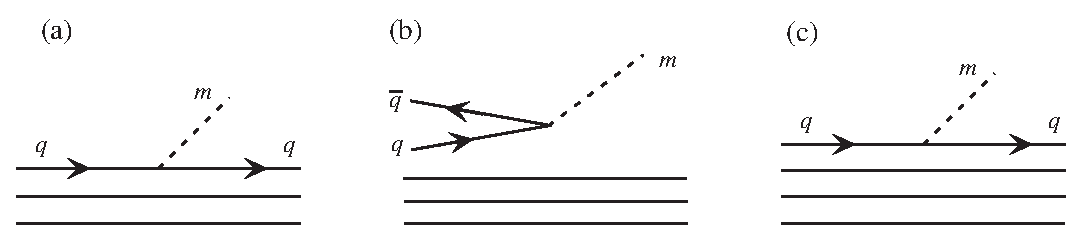
\includegraphics[width=14cm,clip]{fig_decay.eps}
\caption{
Caption Caption Caption Caption Caption Caption Caption Caption Caption  }
\label{fallapart}
\end{figure}
%figure---------------------------------------------


Discussions Discussions Discussions Discussions Discussions Discussions Discussions Discussions 
Discussions Discussions Discussions Discussions Discussions Discussions Discussions Discussions 
Discussions Discussions Discussions Discussions Discussions Discussions Discussions Discussions 

%---------------------------------------------
\begin{table}[h]
\centering
\caption{\label{widthp} \small Caption Caption Caption Caption Caption Caption Caption Caption Caption.  
}
\begin{tabular}{ c c | c c c c }
\hline
 &  & \multicolumn{4}{c}{$g_{KNR}$} \\
 &  & $J^P=1/2^-$ & & $1/2^+$ \\
\hline
$\bra r^2 \ket^{1/2}$ &  $\alpha_0^2$  &  & SF  &  SC  &  JW\\
$1/\sqrt{2}$ fm & 3 fm$^{-2}$ & 4.1 & 7.7 & 5.5 & 3.2\\
1 fm & 1.5 fm$^{-2}$ & 3.2 & 8.4 & 5.9 & 3.4\\
\hline
\end{tabular}
\end{table}
%---------------------------------------------

More Discussions More Discussions More Discussions More Discussions More Discussions More Discussions
More Discussions More Discussions More Discussions More Discussions More Discussions More Discussions



%=============================================
% In the environment {thebibliography} below, 
% DO NOT REMOVE \vspace*{-0.2cm}
%=============================================

\begin{thebibliography}{9}
%
\vspace*{-0.2cm}
\bibitem{Brambilla:2022ura}
N.~Brambilla, H.~X.~Chen, A.~Esposito, J.~Ferretti, A.~Francis, F.~K.~Guo, C.~Hanhart, A.~Hosaka, R.~L.~Jaffe and M.~Karliner, \textit{et al.}
%``Substructure of Multiquark Hadrons (Snowmass 2021 White Paper),''
[arXiv:2203.16583 [hep-ph]].

\vspace*{-0.2cm}

\bibitem{Aoki:2021cqa}
K.~Aoki, H.~Fujioka, T.~Gogami, Y.~Hidaka, E.~Hiyama, R.~Honda, A.~Hosaka, Y.~Ichikawa, M.~Ieiri and M.~Isaka, \textit{et al.}
%``Extension of the J-PARC Hadron Experimental Facility: Third White Paper,''
[arXiv:2110.04462 [nucl-ex]].

\end{thebibliography}
\end{document}